\subsection{Problems to be addressed}
\label{subsec:problems-to-be-addressed}

This section outlines the potential problems during the research and how to address them.
Each subsection represents a problem, with a brief description of the problem and how to address it.

\subsubsection{How to measure memory usage}

One of the primary challenges is accurately measuring memory usage.
This critical feature that describes the current state of the environment is necessary during the execution of the reinforcement learning model.
Considering the usage of \ac{GPU} memory, this problem may be even more complicated since it would require strategies that may differ from \ac{CPU} memory.

Addressing this issue involves investigating if there is an API to measure \ac{GPU} memory consumption and, if not, exploring standard libraries that allow gathering memory consumption based on a specific process.

\subsubsection{Historical data requirements}

Many current approaches require significant historical data to train the models.
Those are not feasible for this research since each execution graph would require a different data set to train the models.

Using a reinforcement learning approach will allow us to overcome this limitation.
This approach will allow the model to learn from the data during execution, learning from its mistakes and improving its predictions.
Figure \ref{fig:reinf-learning} shows a diagram illustrating how this approach will work.
The agent will evaluate the current state, considering both input-related features as well as memory usage since the algorithm started, and will take an action that could be:
(i) \textit{continue} to execute the algorithm with the current chunk size;
(ii) \textit{rechunk} the data to a different chunk size;
or (iii) \textit{reset} the execution of the algorithm with a different initial chunk size.

The interpreter will evaluate the agent's actions and provide a reward based on memory usage efficiency.

\begin{figure}[ht]
  \caption{Reinforcement learning execution diagram}
  \label{fig:reinf-learning}
  \resizebox{\textwidth}{!}{%
    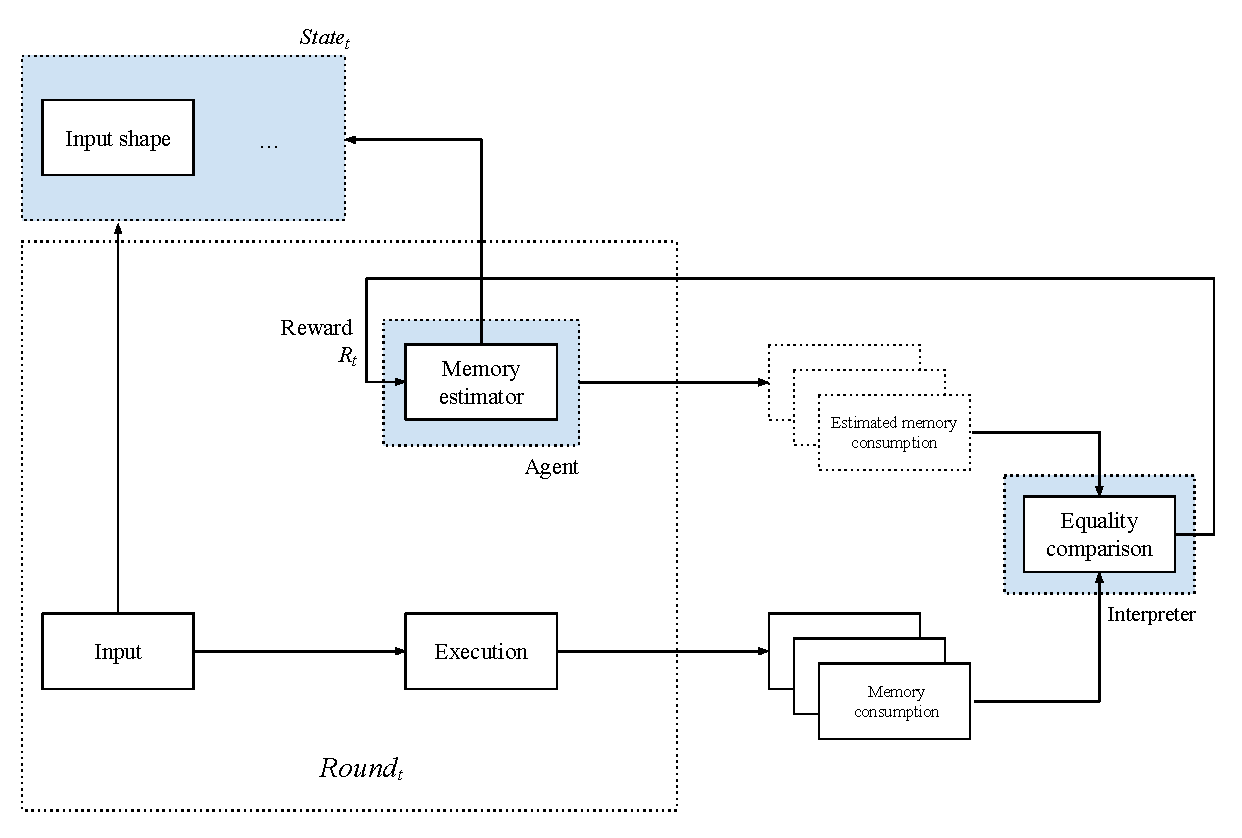
\includegraphics{usage-diagram.pdf}
  }
\end{figure}

\subsubsection{Python's garbage collection}

Python's garbage collector can pose a problem for this research.
Python uses reference counting as its garbage collection strategy. It is lazy and usually waits for the necessary memory to collect the garbage and free memory space.
If the operators are \ac{CPU} memory bounded, it would be necessary to figure out how to deal with Python's garbage collector to gather memory usage when collecting memory consumption information.

\subsubsection{Graph execution}

Another possible problem is figuring out the entire graph's memory requirements.
While the proposed solution allows controlling the chunk size of a specific algorithm, integrating multiple algorithms into a graph poses a challenge.
Nevertheless, it is crucial to understand how to abstract the model agent to persist the state during the graph execution.
